\chapter{Revisão Bibliográfica} \label{ch:soa}
\setlength{\headheight}{13.6pt}
%%%%%%%%%%%%%%%%%%%%%%%%%%%%%%%%%%%%%%%%%%%%%%%%%%%%%%%%%%%%%%%%%%%%%%%%%%%%%
\section{Caixas de Velocidade} \label{sec:soa_caixas}
Uma caixa de velocidades é um componente em veículos com motor que é responsável por transmitir a potência do motor para as rodas, permitindo controlar a velocidade e o torque do veículo. Para isso, são utilizados um conjunto de engrenagens que podem ser engatadas ou desengatadas para alterar a relação de transmissão entre o motor e as rodas. Essas engrenagens, são divididas em mudanças, que determinam a relação entre a rotação do motor e a velocidade do veículo. O diferencial, por outro lado, é um componente cuja função principal é distribuir a potência vinda da caixa de velocidades de forma adequada entre as rodas de um mesmo eixo, permitindo que elas girem em velocidades diferentes durante curvas, garantindo a estabilidade e o controlo do veículo. O diferencial pode estar localizado no veio de transmissão das rodas, ou, como é o caso das caixas de velocidade produzidas com os componentes que são escopo desta tese, também pode estar incorporado na caixa de velocidades, e é constituído por uma roda de coroa e por engrenagens planetárias, que transmitem a potencia para as rodas.
%%%%%%%%%%%%%%%%%%%%%%%%%%%%%%%%%%%%%%%%%%%%%%%%%%%%%%%%%%%%%%%%%%%%%%%%%%%%%
\begin{figure}[htb]
    \centering
    \begin{subfigure}{.5\textwidth}
        \centering
        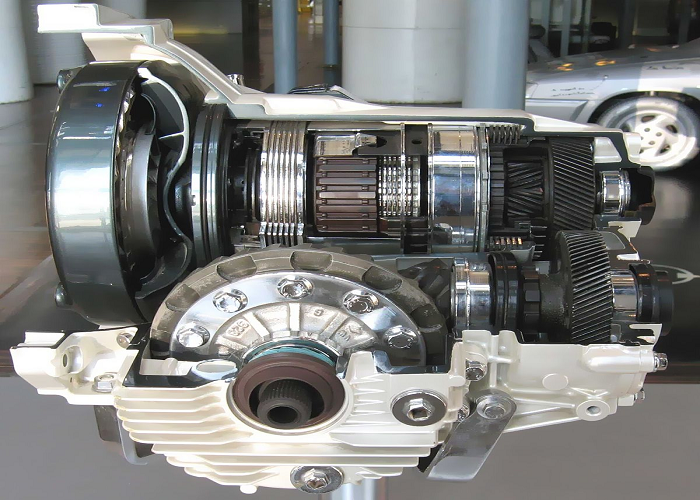
\includegraphics[width = 0.9\textwidth]{Figures/Cap2/Caixa_de_velocidades.png}
        \caption{}
        \label{fig:caixa_de_velocidades}
    \end{subfigure}%
    \begin{subfigure}{.5\textwidth}
        \centering
        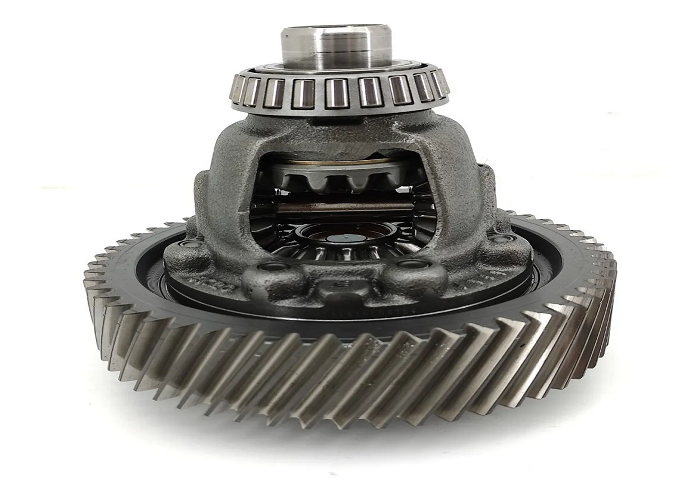
\includegraphics[width = 0.9\textwidth]{Figures/Cap2/Caixa_diferencial.png}
        \caption{}
        \label{fig:diferencial_montado}
    \end{subfigure}
\caption[Uma caixa de velocidades e uma caixa diferencial]%
{À esquerda, uma fotografia de uma caixa de velocidades JT4 aberta para ensaio. À direita, um veio diferencial DB45 com as engrenagens planetárias, antes de ser montada numa caixa de velocidades.}
\end{figure}
%%%%%%%%%%%%%%%%%%%%%%%%%%%%%%%%%%%%%%%%%%%%%%%%%%%%%%%%%%%%%%%%%%%%%%%%%%%%%
\newpage
\par
Uma engrenagem é um sistema mecânico que consiste em duas rodas dentadas que se interligam para transmitir o movimento entre elas. No âmbito deste trabalho, diretamente ligado à transmissão de movimento, as duas rodas dentadas transmitem potência por contacto mutuo da superfície dos dentes conjugados. Uma engrenagem é composta por um pinhão, a roda mais pequena, que pode estar associada a uma roda, uma cremalheira, uma coroa ou um parafuso sem-fim.
\par
Dos modos de solicitação nos dentes das engrenagens, os mais importantes são a flexão do dente devido ao momento fletor na base do dente gerado pela força de engrenamento e as tensões de Hertz, geradas pelo contacto mútuo entre flancos de dois dentes engrenados \cite{Completo2019}.
%%%%%%%%%%%%%%%%%%%%%%%%%%%%%%%%%%%%%%%%%%%%%%%%%%%%%%%%%%%%%%%%%%%%%%%%%%%%%
\begin{figure}[htb]
    \centering
    \begin{subfigure}{.5\textwidth}
        \centering
        \includegraphics[width = 0.9\textwidth]{Figures/Cap2/Completo_rodas.png}
        \caption{}
        \label{fig:dentes elicoidais}
    \end{subfigure}%
    \begin{subfigure}{.5\textwidth}
        \centering
        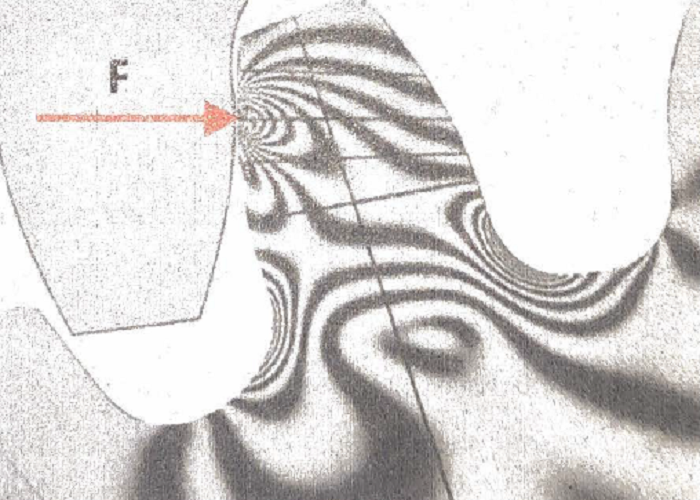
\includegraphics[width = 0.9\textwidth]{Figures/Cap2/Completo2019.png}
        \caption{}
        \label{fig:franjas_fotoelásticas}
    \end{subfigure}
\caption[Engrenagem de eixos paralelos e um padrão de franjas fotoelásticas]%
{À esquerda, uma engrenagem de eixos paralelos e dentes helicoidais.À direita, um padrão de franjas fotoelásticas referente ao gradiente de tensão de dentado reto.\cite{Completo2019}.}
\end{figure}
%%%%%%%%%%%%%%%%%%%%%%%%%%%%%%%%%%%%%%%%%%%%%%%%%%%%%%%%%%%%%%%%%%%%%%%%%%%%%
\par  
Enquanto a flexão do dente é tão maior quanto maior a sua tenacidade, a Resistência ao Contacto, pelas tensões de Hertz, segue o caminho oposto, sendo esta fortemente ligada à dureza. A tenacidade geralmente segue uma relação inversa com a dureza, portanto, um material muito duro, geralmente tem baixa tenacidade.
Dito isto, é então importante ser realizado um Tratamento na Superfície de Contacto entre a engrenagem, para lhe conferir uma maior dureza superficial sem interferir na capacidade do pé do dente de absorver energia de deformação, adquirindo às rodas dentadas bons coeficientes de resistência tanto em relação aos dois modos de solicitação. Além disso, é interessante que a superfície de contacto entre a roda dentada e o veio de transmissão de potência não sofra tratamento, sendo esta ‘interface’ estática, é idealmente pretendido uma maior tenacidade, pelo que é importante minimizar, nesta superfície, as ações sofridas pelo tratamento térmico realizado na roda dentada.
\newpage
%%%%%%%%%%%%%%%%%%%%%%%%%%%%%%%%%%%%%%%%%%%%%%%%%%%%%%%%%%%%%%%%%%%%%%%%%%%%%
\section{Tratamentos Térmicos} \label{sec:soa_tratamentos}
%%%%%%%%%%%%%%%%%%%%%%%%%%%%%%%%%%%%%%%%%%%%%%%%%%%%%%%%%%%%%%%%%%%%%%%%%%%%%
\subsection{Têmpera} \label{ssec:soa_tratamentos_tempera}

Têmpera é o arrefecimento rápido de uma peça metálica em água, óleo, polímero líquido, ou outros fluidos para obter determinadas propriedades dos materiais onde se visa evitar a ocorrência de processos como transformações de fase. Isto é possível ao imergir a peça metálica num fluido a baixa temperatura, aumentando rapidamente o gradiente de temperaturas entre a superfície da peça e o meio externo e diminuindo o tempo em que o material está às temperaturas favoráveis às transformações de fase\cite{Chaus2006}.O seu termo em inglês é “Quenching” e não deve ser confundido com “Tempering”, que em português traduz-se por Revenido.
%%%%%%%%%%%%%%%%%%%%%%%%%%%%%%%%%%%%%%%%%%%%%%%%%%%%%%%%%%%%%%%%%%%%%%%%%%%%%
\par
O mecanismo de obtenção de uma têmpera num aço, requer que seja atingida uma temperatura de austenitização, portanto, esta temperatura é intrínseca de cada liga(Ver Figura \ref{fig:Iron_Carbon_Diagram}). Geralmente, uma temperatura cerca de 50 \textdegree C acima da temperatura teórica é mantida durante algumas horas de forma a assegurar que há uma transformação total da microestrutura do aço da liga.
%%%%%%%%%%%%%%%%%%%%%%%%%%%%%%%%%%%%%%%%%%%%%%%%%%%%%%%%%%%%%%%%%%%%%%%%%%%%%
\begin{figure}[htb]
    \centering
    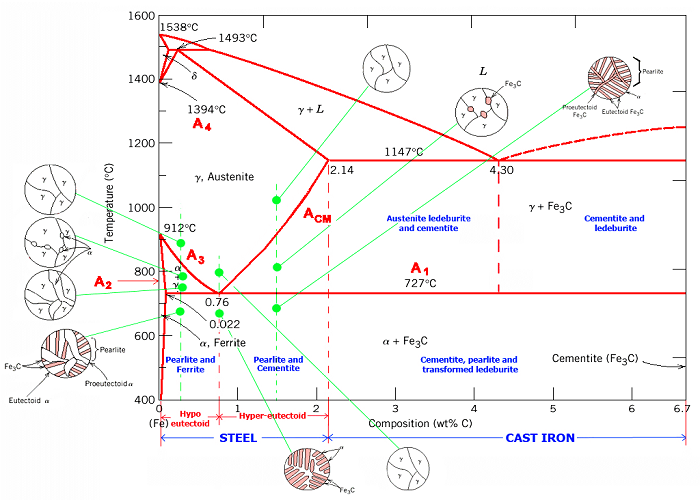
\includegraphics[width = 0.6\textwidth]{Figures/Cap2/Iron_Carbon_Diagram.png}
    \caption[Gráfico de fases do aço. Carbono x Ferro]%
    {Gráfico de fases do aço sem elementos de liga. Carbono x Ferro\cite{FollSD}. }
    \label{fig:Iron_Carbon_Diagram}
\end{figure}
%%%%%%%%%%%%%%%%%%%%%%%%%%%%%%%%%%%%%%%%%%%%%%%%%%%%%%%%%%%%%%%%%%%%%%%%%%%%%
\par
Uma vez que o aço tenha atingido a temperatura de austenitização, este é arrefecido rapidamente, de forma a evitar a etapa de transformação da microestrutura e impedindo a austenite de voltar ao estado de ferrite, estado de estabilidade da microestrutura do aço à temperatura ambiente. Uma vez que a obtenção da microestrutura final não seria possível sem o uso de um mecanismo como a têmpera, este tipo de microestrutura é chamada “microestrutura metastável”, e denomina-se martensite.
%%%%%%%%%%%%%%%%%%%%%%%%%%%%%%%%%%%%%%%%%%%%%%%%%%%%%%%%%%%%%%%%%%%%%%%%%%%%%
\par
Uma consequência da instabilidade da martensite, é que esta pode ser transformada noutros tipos de microestruturas mais estáveis, uma vez que se atinja uma temperatura que possibilite tal ocorrência. Uma das finalidades da têmpera, o aumento da dureza e da resistência, é obtido devido a esta alteração da microestrutura, uma vez que o tamanho dos grãos de martensite é menor que os grãos de ferrite, aumenta-se consequentemente a dureza\cite{Krauss2015}. Outro motivo para o aumento da dureza deve-se ao nível de tensões internas nos grãos de martensite é extremamente elevado, devido à natureza da disposição dos átomos nas duas microestruturas cristalinas. (Ver Figura \ref{fig:Crystal})
%%%%%%%%%%%%%%%%%%%%%%%%%%%%%%%%%%%%%%%%%%%%%%%%%%%%%%%%%%%%%%%%%%%%%%%%%%%%%
\begin{figure}[htb]
    \centering
    \begin{subfigure}{.5\textwidth}
      \centering
      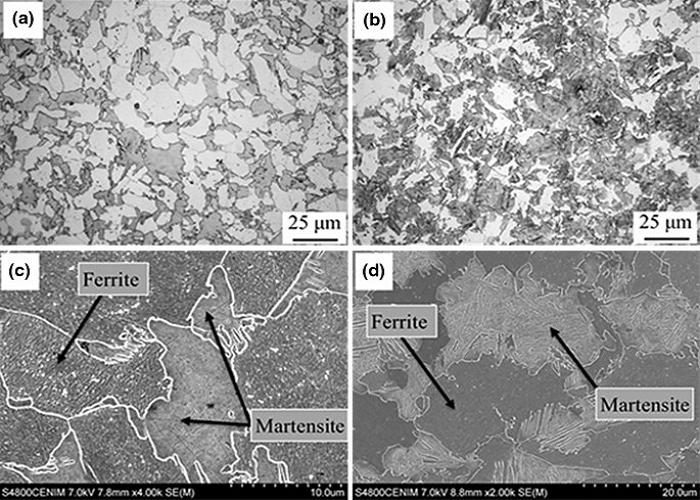
\includegraphics[width = 0.9\textwidth]{Figures/Cap2/Ferrite_Martensite.png}
      \caption{}
      \label{fig:Crystal}
    \end{subfigure}%
    \begin{subfigure}{.5\textwidth}
      \centering
      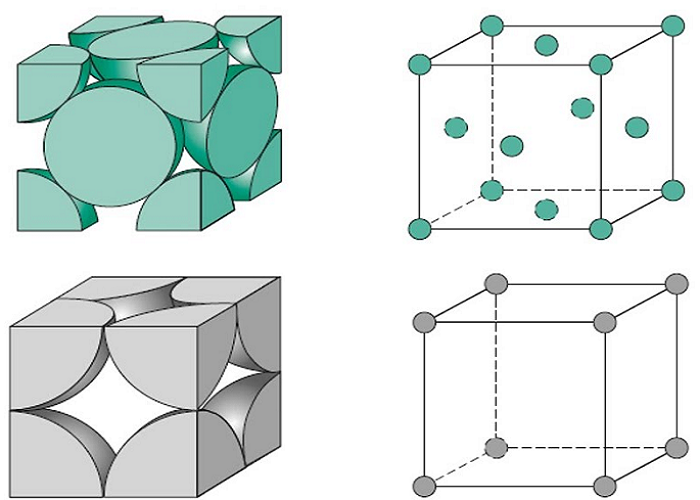
\includegraphics[width = 0.9\textwidth]{Figures/Cap2/CFC_CS.png}
      \caption{}
      \label{fig:CFC_CS}
    \end{subfigure}
\caption[Diferenças entre microestruturas de martensite e ferrite]%
{À esquerda, uma imagem microscópica dos grãos de ferrite e martensite, respetivamente indicados por meio de setas nas figuras. À direita, respetivamente de cima para baixo, a estrutura cristalina CFC da martensite, e a estrutura cristalina CS da ferrite.}
\end{figure}
%%%%%%%%%%%%%%%%%%%%%%%%%%%%%%%%%%%%%%%%%%%%%%%%%%%%%%%%%%%%%%%%%%%%%%%%%%%%%
\par
Outra razão para o aumento da dureza e da resistência, é que a martensite tem uma estrutura cúbica de face centrada(Ver Figura \ref{fig:CFC_CS}), ao contrário da ferrite, que é cúbica simples, sendo assim limitada nos graus de liberdade disponíveis sob os quais os átomos podem deslocar-se de uma estrutura cristalina para outra.
%%%%%%%%%%%%%%%%%%%%%%%%%%%%%%%%%%%%%%%%%%%%%%%%%%%%%%%%%%%%%%%%%%%%%%%%%%%%%
%%%%%%%%%%%%%%%%%%%%%%%%%%%%%%%%%%%%%%%%%%%%%%%%%%%%%%%%%%%%%%%%%%%%%%%%%%%%%
\begin{figure}[htb]
    \centering
    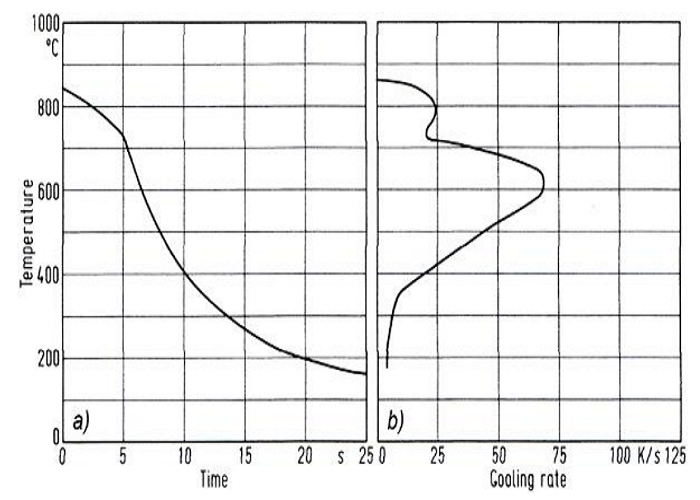
\includegraphics[width = 0.6\textwidth]{Figures/Cap2/Tempera_Arrefecimento.png}
    \caption[Curva de arrefecimento em fluido de têmpera]%
    {Curvas de arrefecimento de uma peça imersa num fluido de têmpera.}
    \label{fig:tempera_arref}
\end{figure}
%%%%%%%%%%%%%%%%%%%%%%%%%%%%%%%%%%%%%%%%%%%%%%%%%%%%%%%%%%%%%%%%%%%%%%%%%%%%%
\par
No entanto, a microestrutura resultante e as propriedades mecânicas associadas dependem da taxa de arrefecimento obtida durante o processo de têmpera. Na curva de arrefecimento da Figura \ref{fig:tempera_arref}, podem ser verificadas três fases de arrefecimento. A primeira consiste no arrefecimento por meio de uma camada de vapor, onde a maior parte do calor é transferida por radiação. Esta camada é formada por um fenómeno chamado \textbf{“Efeito Leidenfrost”}, que ocorre quando um líquido entra em contacto com uma superfície significativamente mais quente do que seu ponto de ebulição. 
\newpage
\par
Nesse caso, uma camada de vapor é formada entre a superfície e o líquido, o que cria um isolamento térmico que impede a evaporação completa do líquido. Isso faz com que este “flutue” sobre a superfície, criando uma barreira de vapor que reduz a transferência de calor entre a superfície e o líquido. A segunda fase, que conta com a convecção como maior meio de transporte de calor, consiste no arrefecimento por transporte de vapor. Como já não se verifica a ocorrência do efeito Leidenfrost, é possível uma livre evaporação do fluido de têmpera, o que aumenta a velocidade de convecção, e por consequência, a velocidade de arrefecimento. A última fase, no entanto, dá-se quando a superfície já se encontra numa temperatura abaixo da temperatura de transformação de fase liquido-vapor do fluido, portanto a velocidade relativa do líquido é muito mais baixa que na segunda fase, e por consequência, a velocidade de arrefecimento significativamente mais baixa.

%%%%%%%%%%%%%%%%%%%%%%%%%%%%%%%%%%%%%%%%%%%%%%%%%%%%%%%%%%%%%%%%%%%%%%%%%%%%%
\subsection{Revenido} \label{ssec:soa_tratamentos_revenido}

O Revenido é um tipo de tratamento térmico normalmente utilizado após tratamento de Tempera que consiste em aquecer e manter o material até uma certa temperatura, abaixo da temperatura crítica, para então resfriar-se ao ar, e desta forma aliviar tensões residuais, diminuir dureza e aumentar tenacidade\cite{Krauss2015}. A combinação de um Revenido a seguir de uma Tempera também é conhecida como “Q\&T Treatment”.
%%%%%%%%%%%%%%%%%%%%%%%%%%%%%%%%%%%%%%%%%%%%%%%%%%%%%%%%%%%%%%%%%%%%%%%%%%%%%
\par
Aços tratados termicamente formam microestruturas martensíticas, que tem maior dureza, força, resistência à fadiga e desgaste resistência quando comparadas a microestruturas de ferrite, no entanto, estruturas martensíticas obtidas por têmpera tem baixa resistência à fratura e tenacidade\cite{Krauss2001}. Uma vez que o tratamento de aços com microestruturas martensíticas são tradicionalmente monitorados por medições de dureza, é importante demonstrar que existe uma relação entre a temperatura do revenido, a quantidade de carbono do aço e a sua dureza final(Ver \textbf{Figura}\ref{fig:Hardness_Temperature_Carbon}). Consequentemente, a quantidade de microestruturas martensíticas e a resistência à fratura e tenacidade do aço que sobre o revenido depende da temperatura do processo.
\par
Tipicamente, as temperaturas de revenido rondam os (150 – 400) \textdegree C, onde o objetivo é reter a maioria das estruturas martensíticas. Em geral, qualquer temperatura pode ser utilizada ao se realizar um revenido, no entanto, as temperaturas mais utilizadas normalmente conferem boa relação entre as propriedades adquiridas pela tempera, sem abdicar da resistência à fratura e tenacidade do material.
%%%%%%%%%%%%%%%%%%%%%%%%%%%%%%%%%%%%%%%%%%%%%%%%%%%%%%%%%%%%%%%%%%%%%%%%%%%%%
\begin{figure}[htb]
    \centering
    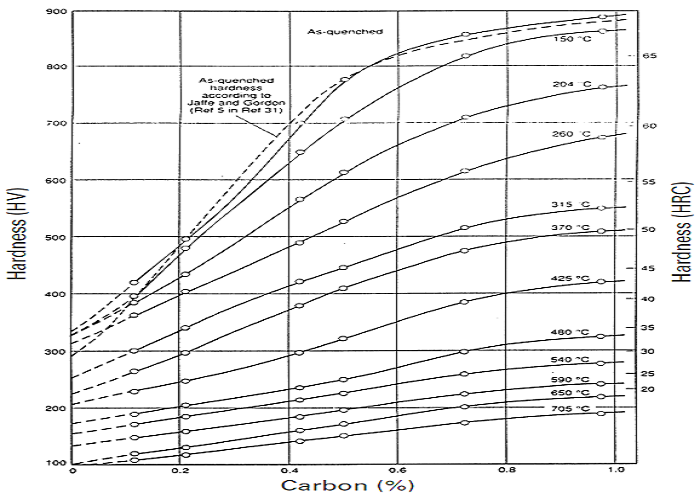
\includegraphics[width = 0.6\textwidth]{Figures/Cap2/Hardness_Temperature_Carbon.png}
    \caption[Relação Revenido: Dureza x Temperatura]%
    {Relação entre temperatura, quantidade de carbono e a dureza de um aço após um revenido\cite{Krauss2001}.}
    \label{fig:Hardness_Temperature_Carbon}
\end{figure}
%%%%%%%%%%%%%%%%%%%%%%%%%%%%%%%%%%%%%%%%%%%%%%%%%%%%%%%%%%%%%%%%%%%%%%%%%%%%%
\subsection{Cementação} \label{ssec:soa_tratamentos_cementação}

Cementação ou carburação é um tratamento termoquímico que consiste em se introduzir carbono na superfície do aço, o que pode ser feito por meio de uma atmosfera controlada, rica em carbono, visando-se aumentar a dureza superficial do material. O mecanismo de ação da cementação é idêntico ao da carbonitruração, que será abordado na \textbf{\ref{ssec:soa_tratamentos_carbonitruracao}}. Com este tipo de tratamento, é possível aumentar superficialmente a percentagem de carbono no aço, aumentando a quantidade de microestrutura martensítica, consequentemente aumentando a dureza desta superfície, com interferências marginais no núcleo da peça tratada \cite{Oberg1989}.

%%%%%%%%%%%%%%%%%%%%%%%%%%%%%%%%%%%%%%%%%%%%%%%%%%%%%%%%%%%%%%%%%%%%%%%%%%%%%
\subsection{Nitruração}

De forma análoga à \textbf{Cementação}, a Nitruração é um tratamento termoquímico que visa a introdução de Azoto na superfície do aço. Também pode ser feita por meio de uma atmosfera controlada. O objetivo da introdução do azoto é criar uma distorção na rede cristalina da microestrutura de forma a aumentar a dureza e modificar outras características do material, superficialmente. Um estudo da microestrutura, feito por meio da utilização da espectroscopia de energia dispersiva (EDS, em ingles “Energy Dispersive Spectroscopy”), em raios-x mostra a composição da camada de tratamento térmico, numa região de dimensões (112 × 140) $\mu$ m junto à borda do material, onde a superfície tratada tem aproximadamente (40 – 45) $\mu$m de comprimento onde é maioritariamente composta por ligas de ferro-azoto, que por no que lhe concerne, até o comprimento de (20 – 25) $\mu$ m, é maioritariamente composta por Fe\textsubscript{3}N \cite{EDAX2023}, como pode ser visto na Figura \ref{fig:Nitriding_3_microstructure}.
%%%%%%%%%%%%%%%%%%%%%%%%%%%%%%%%%%%%%%%%%%%%%%%%%%%%%%%%%%%%%%%%%%%%%%%%%%%%%
\begin{figure}[htb]
    \centering
    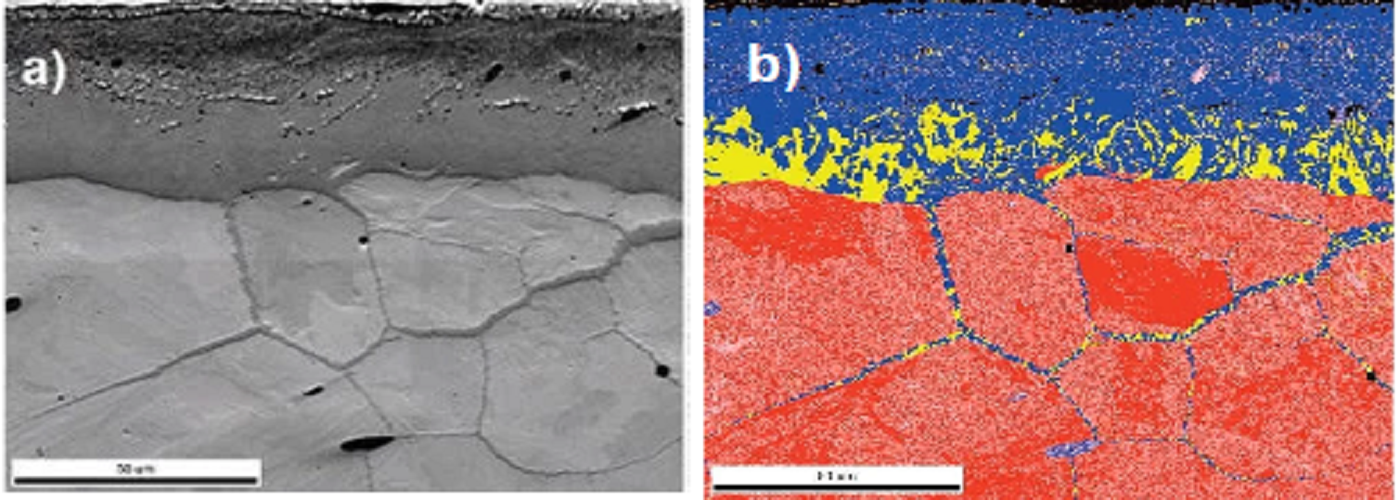
\includegraphics[width = 0.9\textwidth]{Figures/Cap2/Nitriding_3_microstructure.png}
    \caption[Microestruturas de uma peça tratada por nitruração]%
    {Imagens mostrando diferentes contrastes microestruturais na proximidade da superfície da peça tratada\cite{EDAX2023}, e o mapa de fases recolhido com as diversas microestruturas. Em vermelho, ferrite; em azul, Fe\textsubscript{4}N; em amarelo Fe\textsubscript{3}N; e em cor-de-rosa, MnS\textsubscript{2}.}
    \label{fig:Nitriding_3_microstructure}
\end{figure}
%%%%%%%%%%%%%%%%%%%%%%%%%%%%%%%%%%%%%%%%%%%%%%%%%%%%%%%%%%%%%%%%%%%%%%%%%%%%%
\newpage
\par
Outro estudo investigou a influência do tempo de tratamento, a temperatura e o volume de azoto na atmosfera da nitruração de um aço de baixa liga AISI 5140, equivalente ao DIN 41Cr4, e definiu a gama de temperaturas em cerca de (450 – 550)°C para um tempo de tratamento de 1 a 12 horas\cite{Karaoglu2002}. A lista de tempos e temperaturas pode ser vista na \textbf{Tabela} \ref{tab:Nitriding_cond}. Os resultados obtidos podem ser vistos na \textbf{Figura} \ref{fig:Nitriding_gradients}.
%%%%%%%%%%%%%%%%%%%%%%%%%%%%%%%%%%%%%%%%%%%%%%%%%%%%%%%%%%%%%%%%%%%%%%%%%%%%%
\begin{table}[htb]
    \centering
    \caption[Condições dos testes das amostras com vários parâmetros de nitruração]%
    {Condições dos testes dos grupos de amostras\cite{Karaoglu2002}.}
    \label{tab:Nitriding_cond}
    \begin{tabular}{cccc} 
    \toprule
    \textbf{Grupo de amostras} & \textbf{Tempo (h)} & \textbf{Temperatura (°C)} & \textbf{Azoto (vol.\%)}  \\ 
    \hline\hline
    1.500.20                   & 1                  & 500                       & 20                       \\
    4.500.20                   & 4                  & 500                       & 20                       \\
    12.500.20                  & 12                 & 500                       & 20                       \\
    4.450.20                   & 4                  & 450                       & 20                       \\
    4.550.20                   & 4                  & 550                       & 20                       \\
    4.500.60                   & 4                  & 500                       & 60                       \\
    \bottomrule
    \end{tabular}
\end{table}
%%%%%%%%%%%%%%%%%%%%%%%%%%%%%%%%%%%%%%%%%%%%%%%%%%%%%%%%%%%%%%%%%%%%%%%%%%%%%
\begin{figure}[htb]
    \centering
    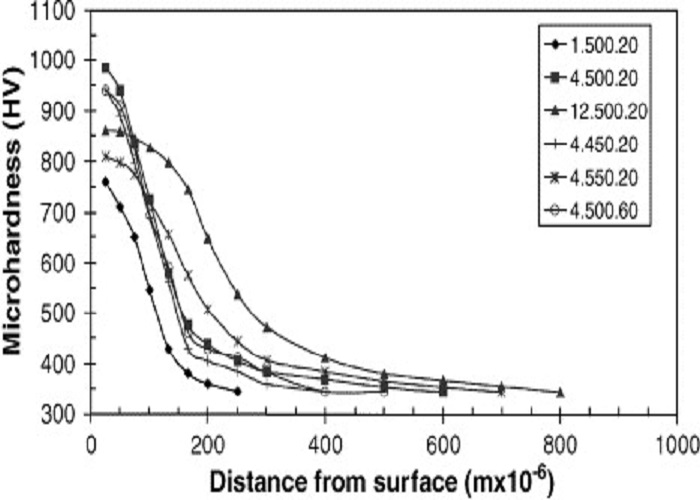
\includegraphics[width = 0.6\textwidth]{Figures/Cap2/Nitriding_gradients.jpg}
    \caption[Durezas obtidas após nitruração]%
    {Valores das durezas obtidas das várias amostras de AISI 5140, para os vários valores de tempo, temperatura e composição da atmosfera\cite{Karaoglu2002}.}
    \label{fig:Nitriding_gradients}
\end{figure}
%%%%%%%%%%%%%%%%%%%%%%%%%%%%%%%%%%%%%%%%%%%%%%%%%%%%%%%%%%%%%%%%%%%%%%%%%%%%%
\par
Destes resultados, é possível identificar uma correlação direta, nesta liga, entre o tempo de carbonitruração e a profundidade da camada tratada, uma vez que para temperaturas e atmosferas semelhantes, o grupo de amostras 1.500.20, com tempo de tratamento de 1 hora, tem dureza a 100 $\mu$ m da superfície de cerca de 550 HV, enquanto o grupo 12.500.20, tem dureza a 100 $\mu$m de cerca de 825 HV. No entanto, as temperaturas, desde que dentro do intervalo estudado, mostram-se pouco relevantes, uma vez que os valores de dureza das amostras com 4 horas de tratamento e 20\% de volume de azoto tem curvas de tensão x profundidade muito semelhantes.
%%%%%%%%%%%%%%%%%%%%%%%%%%%%%%%%%%%%%%%%%%%%%%%%%%%%%%%%%%%%%%%%%%%%%%%%%%%%%
\newpage
\subsection{Carbonitruração} \label{ssec:soa_tratamentos_carbonitruracao}

A carbonitruração, no que lhe concerne, é um processo cujo objetivo é muito semelhante ao da \textbf{Cementação}, e que se diferencia deste uma vez que é adicionado amoníaco (NH\textsubscript{3}) de forma a adicionar azoto à superfície tratada, de forma a melhorar a temperabilidade e possibilitar a formação de martensite em aços de carbono e de baixa liga que inicialmente têm baixa temperabilidade\cite{Herring2011}. Uma das principais vantagens da carbonitruração relativamente à cementação, é que o processo é relativamente mais rápido, conformando uma menor espessura de tratamento, e facilitando a formação de martensite em aços de baixa liga, tornando-o uma escolha altamente rentável para uma vasta gama de aplicações.
Como a cementação, é um processo de tratamento térmico de endurecimento superficial utilizado para melhorar a dureza, resistência ao desgaste e resistência à fadiga de ligas de aço, e ferro fundido, que por sua vez, envolve a difusão de carbono e azoto na superfície do material para formar uma fina camada superficial dura e resistente ao desgaste, enquanto o núcleo do material é mantido dúctil, proporcionando melhores propriedades de superfície, propriedades estas, ideais para a aplicação em questão, uma vez que a coroa é um componente mecânico sujeito a elevados níveis de tensões e desgaste\cite{Bryson2009}. Um exemplo da microestrutura de um aço de baixa liga tratado por carbonitruração pode ser visto na figura \ref{fig:Carbonitriding_microstructure}.
%%%%%%%%%%%%%%%%%%%%%%%%%%%%%%%%%%%%%%%%%%%%%%%%%%%%%%%%%%%%%%%%%%%%%%%%%%%%%
\begin{figure}[htb]
    \centering
    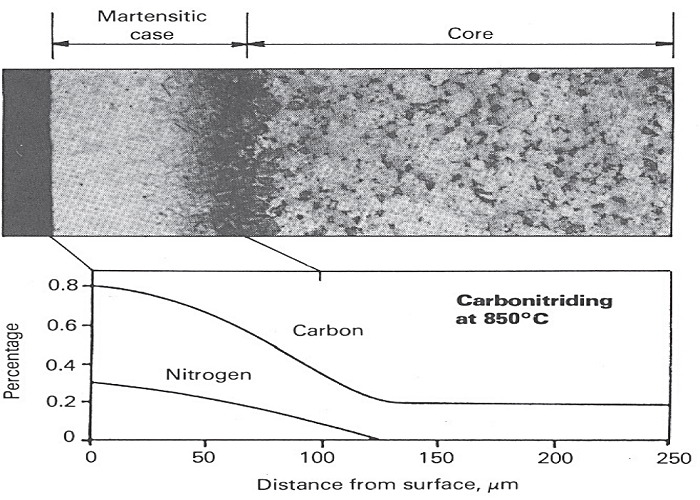
\includegraphics[width = 0.6\textwidth]{Figures/Cap2/Carbonitriding_microstructure.png}
    \caption[Micrografia de uma peça tratada por carbonitruração]%
    {Micrografia das camadas superficiais produzidas por carbonitruração de um aço a 850 \textdegree C. Pode-se observar uma camada martensítica no exterior, e um núcleo predominantemente formado por ferrite\cite{Herring2011}.}
    \label{fig:Carbonitriding_microstructure}
\end{figure}
%%%%%%%%%%%%%%%%%%%%%%%%%%%%%%%%%%%%%%%%%%%%%%%%%%%%%%%%%%%%%%%%%%%%%%%%%%%%
\par
O processo de carbonitruração é realizado ao se aquecer a peça a ser tratada numa atmosfera controlada até uma temperatura por volta de (700 – 900) \textdegree C, num forno de atmosfera controlada que contém Amoníaco (NH\textsubscript{3}) e alguma fonte de Carbono, como, por exemplo, propano (C\textsubscript{3}H\textsubscript{8}), de forma a causar a difusão de carbono e azoto na superfície do metal, formando uma camada que tem tipicamente de 0,5 a 1,5 milímetros de espessura\cite{Rajan2011}, sendo esta profundidade da superfície tratada dependente das condições do processo, incluindo a temperatura, o tempo e a composição da atmosfera. A Figura \ref{fig:Carbonitriding_depth} exemplifica graficamente a dependência entre a profundidade, a temperatura e o tempo.
%%%%%%%%%%%%%%%%%%%%%%%%%%%%%%%%%%%%%%%%%%%%%%%%%%%%%%%%%%%%%%%%%%%%%%%%%%%%
\begin{figure}[htb]
    \centering
    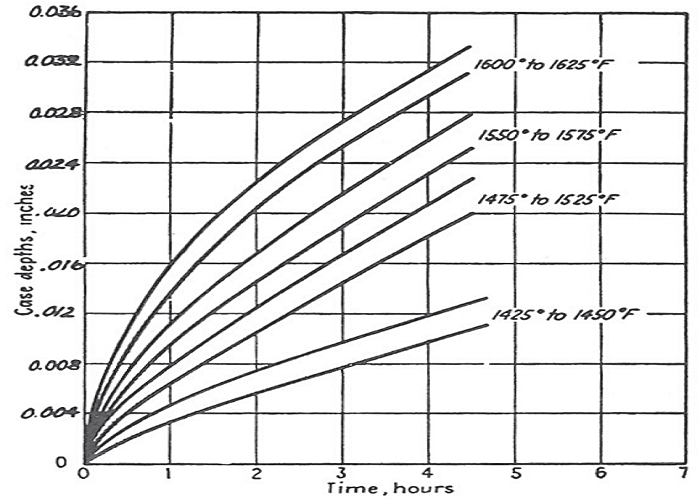
\includegraphics[width = 0.6\textwidth]{Figures/Cap2/Carbonitriding_depth.png}
    \caption[Composição de carbono e azoto em relação à profundidade de tratamento]%
    {Gráfico que mostra a profundidade do tratamento de carbonitruração, em polegadas relativamente ao tempo de tratamento, em horas, para várias temperaturas, em Fahrenheit.\cite{Herring2011}}
    \label{fig:Carbonitriding_depth}
\end{figure}%%%%%%%%%%%%%%%%%%%%%%%%%%%%%%%%%%%%%%%%%%%%%%%%%%%%%%%%%%%%%%%%%%%%%%%%%%%%%
\newpage
\par
Outra correlação importante em peças tratadas por carbonitruração, é a correlação entre a dureza e a taxa percentual de carbono, sendo estas quase diretamente relacionadas, pelo que, uma vez que a dureza da camada é mais baixa, pode-se assumir que a taxa de carbono no ponto também o é, evitando assim que uma análise da micrografia do material, a qual é um ensaio destrutivo, seja feita sempre que se queira verificar a quantidade de carbono depositado no ponto em questão. Esta correlação pode ser visualizada na figura \ref{fig:Carbon_Hardness_Carbonitriding}
%%%%%%%%%%%%%%%%%%%%%%%%%%%%%%%%%%%%%%%%%%%%%%%%%%%%%%%%%%%%%%%%%%%%%%%%%%%%%
\begin{figure}[htb]
    \centering
    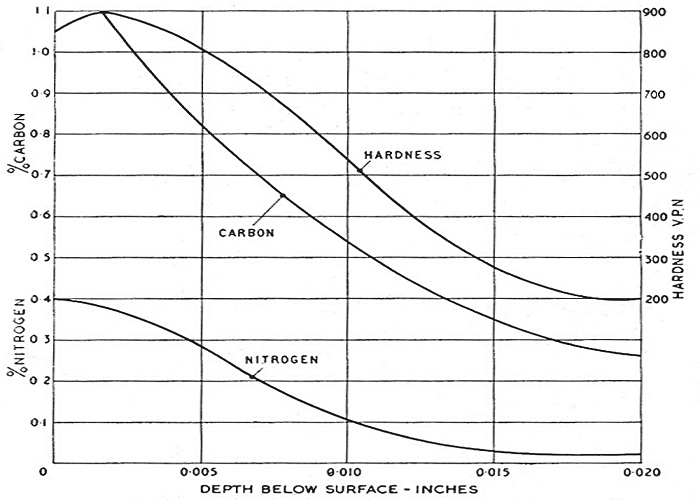
\includegraphics[width = 0.6\textwidth]{Figures/Cap2/Carbon_Hardness_Carbonitriding.png}
    \caption[Relação entre carbono, azoto e dureza]%
    {Gráfico que mostra a relação entre a quantidade de carbono no ponto e a dureza\cite{Herring2011}. Mais uma vez, pode-se observar que a deposição de carbono diminui à medida que a distância da superfície tratada aumenta.}
    \label{fig:Carbon_Hardness_Carbonitriding}
\end{figure}
%%%%%%%%%%%%%%%%%%%%%%%%%%%%%%%%%%%%%%%%%%%%%%%%%%%%%%%%%%%%%%%%%%%%%%%%%%%%%
\newpage
\par
Por fim, a têmpera é um passo essencial após a carbonitruração, uma vez que ajuda a solidificar as posições dos átomos de carbono e azoto adquiridos na etapa da carbonitruração, formando as estruturas martensíticas discutidas no Subcapítulo \ref{ssec:soa_tratamentos_tempera}. Sem uma têmpera, o aço pode não atingir a dureza e resistência desejadas. Evidentemente, uma vez que a superfície que sofreu a carbonitruração tem uma composição de carbono superior à composição do núcleo, esta superfície deve tornar-se mais dura que o núcleo, mas será maioritariamente composta por ferrite, que, ao contrário da martensite, não confere uma dureza tão elevada ao material. É importante evidenciar que, mesmo que não seja feita uma têmpera, o aço tratado ainda poderá ter elevados níveis de deformações originadas pela energia térmica obtida na etapa de adsorção de carbono e azoto, porquanto a superfície tem uma composição química ligeiramente diferente do núcleo, o que pode ocasionar diferentes gradientes de temperatura e diferentes deslocamentos. Por conseguinte, é essencial que sejam seguidas as etapas adequadas do tratamento térmico, para serem alcançadas as propriedades desejadas e assegurar a obtenção do produto final.
%%%%%%%%%%%%%%%%%%%%%%%%%%%%%%%%%%%%%%%%%%%%%%%%%%%%%%%%%%%%%%%%%%%%%%%%%%%%%
\section{Soldadura}\label{sec:soldadura}
%%%%%%%%%%%%%%%%%%%%%%%%%%%%%%%%%%%%%%%%%%%%%%%%%%%%%%%%%%%%%%%%%%%%%%%%%%%%%
\subsection{Soldabilidade de aços-carbono}\label{ssec:soldadura-soldabilidade}

A soldadura de metais e ligas é um processo crucial na confeção de caixas de velocidade. No entanto, a soldabilidade de diferentes ligas pode ser afetada pelo percentual de  \textbf{carbono equivalente} — em inglês “Carbon Equivalent”, ou CE — da liga, a qual é uma medida da soldabilidade de uma liga que tem em conta não só a percentagem de carbono como também outros elementos de liga. Existe alguma investigação sobre o impacto da CEP na soldabilidade, reiterando a importância de controlar a quantidade de carbono nas zonas onde serão realizados processos de soldadura.
\par
A Equação \ref{eq:CE-IIW}, foi desenvolvida por Dearden and O'Neill e adotada pelo Instituto Internacional de Soldadura em 1967, sendo considerada adequada para prever a temperabilidade numa grande variedade de aços de carbono simples e aços carbono-manganês, mas não para aços microligados de alta resistência de baixa liga ou aços de baixa liga CrMo. Esta fórmula considera os efeitos combinados do carbono e de outros elementos de liga sobre a temperabilidade do aço. O valor do CE é expresso como uma percentagem, onde os valores de referência em relação à soldabilidade é descrita na Tabela \ref{tab:CE}.
\vspace{5mm}
%%%%%%%%%%%%%%%%%%%%%%%%%%%%%%%%%%%%%%%%%%%%%%%%%%%%%%%%%%%%%%%%%%%%%%%%%%%%%
\begin{equation}
    \centering
    \label{eq:CE-IIW}
    \%C + \frac{\%Mn}{6}+\frac{\%Cr+\%Mo+\%V}{5}+\frac{\%Cu+\%Ni}{15}
\end{equation}
%%%%%%%%%%%%%%%%%%%%%%%%%%%%%%%%%%%%%%%%%%%%%%%%%%%%%%%%%%%%%%%%%%%%%%%%%%%%%
\vspace{5mm}
\par
O cálculo do CE envolve a adição das percentagens de peso dos vários elementos de liga no aço, sendo cada elemento multiplicado por um fator específico. O total resultante é então adicionado à percentagem de carbono da liga, obtendo-se assim, o valor do percentual CE da liga.
\par
Um percentual de CE mais elevado pode levar a questões como o aumento da porosidade, rachadura, e redução da tenacidade na ZAT (Zona Afetada Termicamente)\cite{Karsamas2003} e um aumento de austenite retida\cite{Park2018}, o que leva ao aumento das tensões internas do material, e pode comprometer a resistência e integridade da estrutura soldada.
\par
Para além do seu impacto na qualidade da soldadura, existe uma relação entre o percentual de  CE e a geometria do cordão de solda em aços com baixo teor de carbono. Um percentual de CE mais elevado leva a formas mais irregulares do granulo e a uma maior probabilidade de “undercutting” — termo utilizado para quando a solda reduz a espessura da secção transversal do metal de base, reduzindo a resistência da soldadura e das peças de trabalho — que podem ser difíceis de reparar e podem aumentar o tempo e os custos de produção.
%%%%%%%%%%%%%%%%%%%%%%%%%%%%%%%%%%%%%%%%%%%%%%%%%%%%%%%%%%%%%%%%%%%%%%%%%%%%%
\begin{table}[htb]
    \centering
    \caption[Valores de referência para a soldabilidade de percentuais CE]%
    {Valores de referência para a soldabilidade de percentuais CE \cite{Vladimir2000}.}
    \label{tab:CE}
    \begin{tabular}{cc} 
    \toprule
    CE              & Soldabilidade  \\ 
    \hline\hline
    0.00\% — 0.35\% & Excelente      \\
    0.36\% — 0.40\% & Ótima          \\
    0.41\% — 0.45\% & Boa            \\
    0.46\% — 0.49\% & Razoável       \\
    0.50\% ou maior & Má             \\
    \bottomrule
    \end{tabular}
\end{table}
%%%%%%%%%%%%%%%%%%%%%%%%%%%%%%%%%%%%%%%%%%%%%%%%%%%%%%%%%%%%%%%%%%%%%%%%%%%%%
\subsection{Fissuração induzida por hidrogénio}\label{ssec:soldadura-fissuracao}

A fissuração induzida pelo hidrogénio é um tipo de corrosão que ocorre em componentes metálicos quando estes são expostos a um ambiente rico em hidrogénio, que ocorre quando há migração de hidrogénio do meio para o metal, que pode ocorrer por fontes externas, tais como proteção catódica ou corrosão assistida por hidrogénio, ou por fontes internas, tais como captação de hidrogénio durante a soldadura. Uma vez dentro do metal, o hidrogénio pode causar uma acumulação de pressão interna, levando à formação de fissuras que podem então propagar-se rapidamente, resultando numa falha completa do componente. Uma vez que a atmosfera no forno para a carbonitruração tem como os seus principais constituintes, o amoníaco (NH\textsubscript{3}) e monóxido de carbono (CO), e sendo a temperatura de dissociação do amoníaco por volta de 500\textdegree C, torna a atmosfera, também, rica em hidrogénio.
%%%%%%%%%%%%%%%%%%%%%%%%%%%%%%%%%%%%%%%%%%%%%%%%%%%%%%%%%%%%%%%%%%%%%%%%%%%%%
\begin{figure}[htb]
    \centering
    \begin{subfigure}{.4\textwidth}
        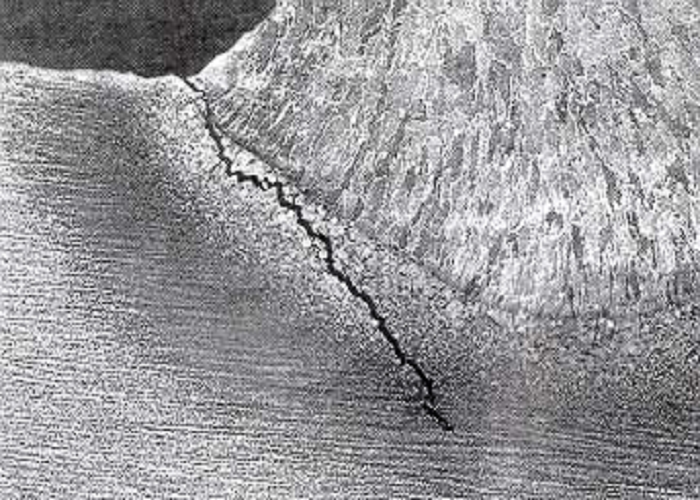
\includegraphics[width = 0.9\textwidth]{Figures/Cap2/Cold_Cracking.png}
        \caption{}
        \label{fig:Fissuracao_1}
    \end{subfigure}%
    \begin{subfigure}{.4\textwidth}
        \centering
        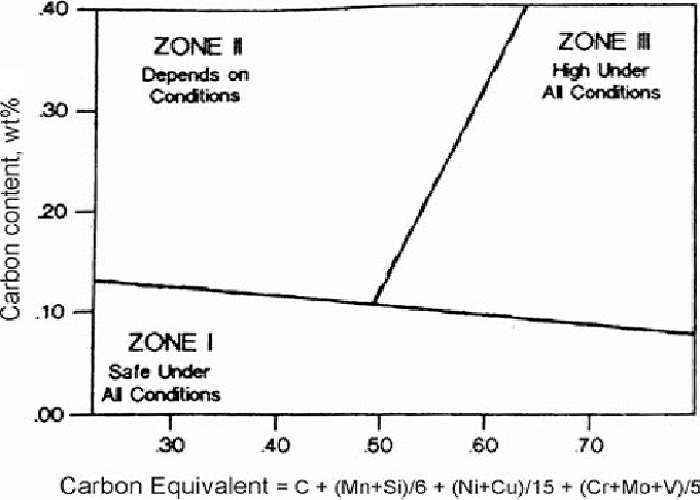
\includegraphics[width = 0.9\textwidth]{Figures/Cap2/Graville_Diagram.png}
        \caption{}
        \label{fig:Graville}
    \end{subfigure}
    \caption[Fissuração induzida por hidrogénio e correlação de Graville]%
    {À esquerda, uma fissuração induzida pelo hidrogénio presente na ZAT (Zona Afetada Termicamente) de uma peça soldada. À direita, correlação de Graville, que correlaciona o percentual de carbono e o percentual de carbono equivalente com ocorrência de fissuras na ZAT (Zona afetada termicamente)\cite{Olson2007}. }
\end{figure}
%%%%%%%%%%%%%%%%%%%%%%%%%%%%%%%%%%%%%%%%%%%%%%%%%%%%%%%%%%%%%%%%%%%%%%%%%%%%%
%%%%%%%%%%%%%%%%%%%%%%%%%%%%%%%%%%%%%%%%%%%%%%%%%%%%%%%%%%%%%%%%%%%%%%%%%%%%%
\begin{figure}[htb]
    \centering
    \begin{subfigure}{.4\textwidth}
      \centering
      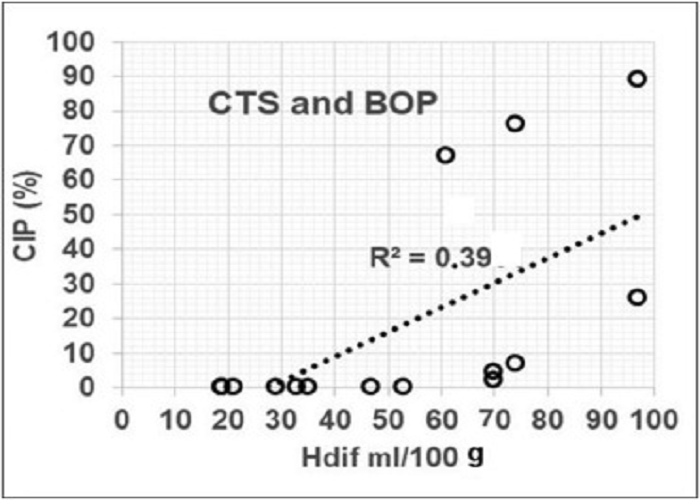
\includegraphics[width = 0.9\linewidth]{Figures/Cap2/Hdif_CE.png}
      \caption{}
      \label{fig:Hdif_CE}
    \end{subfigure}%
    \begin{subfigure}{.4\textwidth}
      \centering
      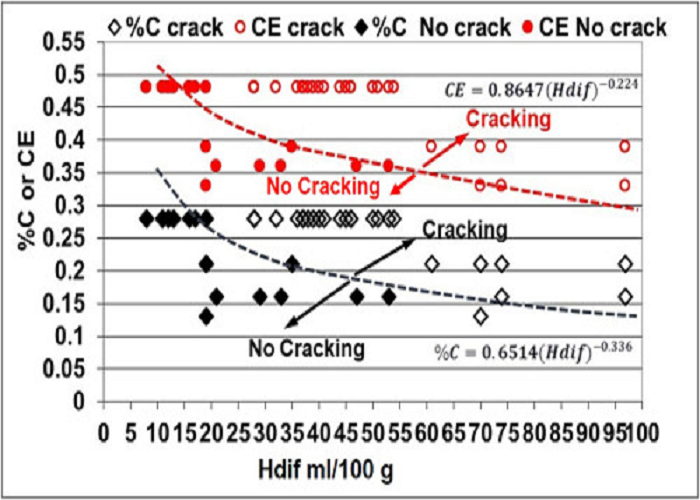
\includegraphics[width = 0.9\linewidth]{Figures/Cap2/CE_Hdif_Crack.png}
      \caption{}
      \label{fig:CE_Hdif_Crack}
    \end{subfigure}
    \caption[Correlações entre hidrogénio difusível e fissuração induzida por hidrogénio]%
    {À esquerda, uma correlação entre o hidrogénio difusível e a ocorrência de fissuração. À direita, uma correlação entre a fissuração a frio, o percentual de carbono ou a taxa CE, e o hidrogénio difusível.}
    \end{figure}
    %%%%%%%%%%%%%%%%%%%%%%%%%%%%%%%%%%%%%%%%%%%%%%%%%%%%%%%%%%%%%%%%%%%%%%%%%%%%%
\newpage
\par
Existe também uma correlação entre o tamanho dos grãos e a facilidade da ocorrência de fissuração\cite{Seo2008}, bem como a quantidade de inclusões não metálicas, como, por exemplo, o Azoto adicionado pelo processo de carbonitruração, isto é, quanto maior o tamanho dos grãos, ou seja, quanto menos espaço houver para a adsorção do hidrogénio, menor é a possibilidade da ocorrência do processo.
\par
De maneira análoga, quanto maior a quantidade de inclusões não metálicas, mais espaço há para a adsorção do hidrogénio, aumentando a possibilidade da ocorrência da fissuração. Um estudo verificou uma correlação entre a quantidade de hidrogénio difusível e a ocorrência de fissuração induzida por hidrogénio\cite{Santos2021} (Ver Figura \ref{fig:Hdif_CE}) em contentores soldados por arco submerso, bem como uma correlação entre a taxa percentual de carbono equivalente, a quantidade de hidrogénio difusível, e a ocorrência de fissuras (Ver Figura \ref{fig:CE_Hdif_Crack}). Com isto, desde que seja possível mensurar a quantidade de hidrogénio difusível, é possível estimar a probabilidade da ocorrência de uma fissura no material.
\par
Para além da relação entre o hidrogénio difusível e a ocorrência de fissuração, existe uma correlação entre o percentual de carbono e de carbono equivalente, denominada “Correlação de Graville”, que correlaciona estes dois valores com a ocorrência de fissuração da ZAT (Zona Afetada Termicamente) (Ver \textbf{Figura} \ref{fig:Graville})\cite{Olson2007}.

%%%%%%%%%%%%%%%%%%%%%%%%%%%%%%%%%%%%%%%%%%%%%%%%%%%%%%%%%%%%%%%%%%%%%%%%%%%%%
\par
Apesar de ainda não existir um mecanismo universalmente aceite para sua deteção, a fissuração por hidrogénio pôde ser correlacionada, nesta aplicação, com duas variáveis que podem ser facilmente medidas ou calculadas. Ainda que o hidrogénio seja muito difícil de detetar no estudo da microestrutura, existem ferramentas que permitem estimar a ocorrência de fissuração por hidrogénio.
%%%%%%%%%%%%%%%%%%%%%%%%%%%%%%%%%%%%%%%%%%%%%%%%%%%%%%%%%%%%%%%%%%%%%%%%%%%%%
\newpage
\subsection{Diagramas da curva de arrefecimento continuo}\label{ssec:diagramas_CCT}
Por fim, é importante mencionar os diagramas CCT (Continuous Cooling Transformation), ou diagramas de curva de arrefecimento contínuo. Estes diagramas mostram as transformações de fase que ocorrem em um material à medida que ele é arrefecido continuamente a partir da temperatura de austenitização e são utilizados para tentar prever as fases que serão formadas de acordo com a velocidade de arrefecimento a que o material for submetido.
\par
As curvas de arrefecimento contínuo são obtidas por meio de ensaios onde o arrefecimento é controlado, onde uma amostra do material é aquecida até a temperatura de austenitização e arrefecida a uma taxa constante. Dependendo da composição química do material, diferentes taxas de arrefecimento podem dar origem a diferentes estruturas finais. A taxa de arrefecimento e a temperatura onde ocorrem as transformações da microestruturas são representadas por meio de curvas, como pode ser visto na Figura \ref{fig:CCT_SOA}.
%%%%%%%%%%%%%%%%%%%%%%%%%%%%%%%%%%%%%%%%%%%%%%%%%%%%%%%%%%%%%%%%%%%%%%%%%%%%%
\begin{figure}[htb]
    \centering
    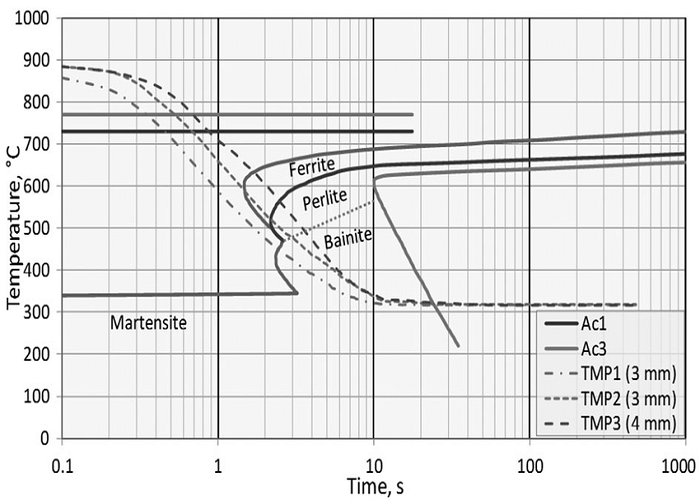
\includegraphics[width = 0.6\textwidth]{Figures/Cap2/CCT_SOA.png}
    \caption[Diagrama CCT de um aço CK45]%
    {Diagrama CCT de um ensaio de arrefecimento de um aço CK45, austenitizado à 880\textdegree C por 5 minutos\cite{Karli2016}.}
    \label{fig:CCT_SOA}
\end{figure}
%%%%%%%%%%%%%%%%%%%%%%%%%%%%%%%%%%%%%%%%%%%%%%%%%%%%%%%%%%%%%%%%%%%%%%%%%%%%%
\par
No entanto, nem sempre é possível realizar um ensaio para a realização de diagramas CCT, pelo que um grupo de pesquisadores tentou modelar por meio de algoritmos de \textit{machine learning}, baseado na composição química, as curvas de arrefecimento contínuo do material \cite{Martin2020}, portanto também é possível tentar prever a microestrutura final do material baseando-se na curva de arrefecimento e composição química. Para além disso, um outro parâmetro extremamente importante na microestrutura final de um material tratado termicamente, é a presença e quantidade de austenite residual, que da-se quando por exemplo, o material é arrefecido a uma taxa de resfriamento inadequada. Se o arrefecimento ocorrer muito rapidamente, a transformação completa da austenite pode ser dificultada.
%%%%%%%%%%%%%%%%%%%%%%%%%%%%%%%%%%%%%%%%%%%%%%%%%%%%%%%%%%%%%%%%%%%%%%%%%%%%%
\newpage
\subsection{Equações para previsão de temperaturas críticas}\label{ssec:previsao_martensite}
Outro fator que pode influenciar a presença de austenite residual é a temperatura de martensite final do material. Sendo esta muito baixa, não há possibilidade de toda a austenite ser transformada em martensite, portanto, resultando numa presença de austenite residual que pode não ser desejada na composição da microestrutura final. Existe, no entanto, uma maneira sugerida para prever as temperaturas de inicio de martensite(M\textsubscript{start}) e fim de martensite(M\textsubscript{finish}) pode ser vista nas Equações \ref{eq:Martensite_start} e \ref{eq:Martensite_finish}, respetivamente\cite{Honeycombe1995}.
%%%%%%%%%%%%%%%%%%%%%%%%%%%%%%%%%%%%%%%%%%%%%%%%%%%%%%%%%%%%%%%%%%%%%%%%%%%%%
\begin{equation}
    \label{eq:Martensite_start}
    \mathrm{M\textsubscript{(start)}}^{\circ}\mathrm{C} = 539-(423\%\mathrm{C})-(30,4\%\mathrm{Mn})-(17.7\%\mathrm{Ni})-(12,1\%\mathrm{Cr})-(7,7\%\mathrm{Mo})
\end{equation}
%%%%%%%%%%%%%%%%%%%%%%%%%%%%%%%%%%%%%%%%%%%%%%%%%%%%%%%%%%%%%%%%%%%%%%%%%%%%%
%%%%%%%%%%%%%%%%%%%%%%%%%%%%%%%%%%%%%%%%%%%%%%%%%%%%%%%%%%%%%%%%%%%%%%%%%%%%%
\begin{equation}
    \label{eq:Martensite_finish}
    \mathrm{M\textsubscript{(finish)}}^{\circ}\mathrm{C} = 346 - (474\%\mathrm{C}) - (33\%\mathrm{Mn}) - (17\%\mathrm{Ni}) - (21\%\mathrm{Mo})
\end{equation}
%%%%%%%%%%%%%%%%%%%%%%%%%%%%%%%%%%%%%%%%%%%%%%%%%%%%%%%%%%%%%%%%%%%%%%%%%%%%%
\par
Também é possível estimar as temperaturas de austenitização inicial(A\textsubscript{C1}) e final (A\textsubscript{C3}) através das equações \ref{eq:A_C1} e \ref{eq:A_C3}, respetivamente\cite{Platl2020}. No entanto, da mesma maneira que as equações para as temperaturas de martensite, estas são apenas estimativas e sempre que possível, deve-se optar pela realização de um ensaio experimental para determinar as temperaturas de transformação da microestrutura.
%%%%%%%%%%%%%%%%%%%%%%%%%%%%%%%%%%%%%%%%%%%%%%%%%%%%%%%%%%%%%%%%%%%%%%%%%%%%%
\begin{equation}
    \label{eq:A_C1}
    \mathrm{A\textsubscript{(C1)}}^{\circ}\mathrm{C} = 723 - (10,7\%\mathrm{Mn}) - (19,9\%\mathrm{Ni}) + (29.1\%\mathrm{Si}) + (6,38\%\mathrm{W})
\end{equation}
%%%%%%%%%%%%%%%%%%%%%%%%%%%%%%%%%%%%%%%%%%%%%%%%%%%%%%%%%%%%%%%%%%%%%%%%%%%%%
%%%%%%%%%%%%%%%%%%%%%%%%%%%%%%%%%%%%%%%%%%%%%%%%%%%%%%%%%%%%%%%%%%%%%%%%%%%%%
\begin{equation}
    \label{eq:A_C3}
    \begin{aligned}
    \mathrm{A\textsubscript{(C3)}}^{\circ}\mathrm{C} = {}   & 910 - (230\sqrt{\%\mathrm{C}}) - (15,2\%\mathrm{Ni}) + (44.7\%\mathrm{Si})\\
                                                            & + (104\%\mathrm{V}) + (31,5\%\mathrm{Mo}) + (6,38\%\mathrm{W})
\end{aligned}
\end{equation}
%%%%%%%%%%%%%%%%%%%%%%%%%%%%%%%%%%%%%%%%%%%%%%%%%%%%%%%%%%%%%%%%%%%%%%%%%%%%%
\par
Essas equações de previsão das temperaturas críticas são desenvolvidas com base em estudos experimentais e modelos termodinâmicos, levando em consideração as composições químicas e as características do material. Com os valores das temperaturas críticas, e com as curvas de transformação de fase mencionadas acima, é possível desenvolver um diagrama CCT estimado, sem a necessidade da realização de ensaios.
%%%%%%%%%%%%%%%%%%%%%%%%%%%%%%%%%%%%%%%%%%%%%%%%%%%%%%%%%%%%%%%%%%%%%%%%%%%%%
\subsection{Equações para previsão de dureza}\label{ssec:previsao_dureza}
Outro uso interessante das velocidades de arrefecimento, para além da previsão da microestrutura final, é a estimativa teórica da dureza final de um aço após um tratamento térmico. Uma estudo apresenta um modelo matemático gerado por um algoritmo computacional para tentar prever a dureza de um aço de acordo com a sua composição química, a velocidade de arrefecimento a que foi submetido, e a microestrutura final\cite{Trzaska2016}. As Equações \ref{eq:HV_fe} e \ref{eq:HV_ma}, indicam a estimativa de dureza consoante a velocidade de arrefecimento e elementos de liga para estruturas ferríticas e martensíticas, respetivamente.
%%%%%%%%%%%%%%%%%%%%%%%%%%%%%%%%%%%%%%%%%%%%%%%%%%%%%%%%%%%%%%%%%%%%%%%%%%%%%
\begin{equation}
    \begin{aligned}
    \mathrm{HV\textsubscript{(ferrite)}} = {}   & -73 + (253\%\mathrm{C}) + (52\%\mathrm{Mn}) + (10\%\mathrm{Si}) + (36\%\mathrm{Cr}) + (8\%\mathrm{Ni})\\
                                                & + (20\%\mathrm{Mo}) + (80\%\mathrm{V}) + (0,11\%\mathrm{A\textsubscript{C1}}) + (12,5\%\mathrm{Vc\textsuperscript{1/4}})
    \end{aligned}
    \label{eq:HV_fe}
\end{equation}
%%%%%%%%%%%%%%%%%%%%%%%%%%%%%%%%%%%%%%%%%%%%%%%%%%%%%%%%%%%%%%%%%%%%%%%%%%%%%
%%%%%%%%%%%%%%%%%%%%%%%%%%%%%%%%%%%%%%%%%%%%%%%%%%%%%%%%%%%%%%%%%%%%%%%%%%%%%
\begin{equation}
    \begin{aligned}
    \mathrm{HV\textsubscript{(martensite)}} = {}    & 200 + (824\sqrt{\%\mathrm{C}}) + (44\%\mathrm{Mn}) + (14\%\mathrm{Cr}) + (9\%\mathrm{Ni})\\
                                                    &+ (171\%\mathrm{V}) + (0,11\%\mathrm{Cu}) + (4,13\%\mathrm{Vc\textsuperscript{1/4}})
    \end{aligned}
    \label{eq:HV_ma}
\end{equation}
%%%%%%%%%%%%%%%%%%%%%%%%%%%%%%%%%%%%%%%%%%%%%%%%%%%%%%%%%%%%%%%%%%%%%%%%%%%%%
\par
Este modelo, claro, tem suas limitações, pelo que está desenvolvido para um intervalo de percentagens de elementos de liga, e tem melhores resultados quando os valores estão mais próximos da média, no entanto, com erros absolutos por volta dos 20-30HVs, esta pode ser uma ferramenta valiosa para a previsão das durezas de um material quando se está a alterar os parâmetros de tratamento. 

%%%%%%%%%%%%%%%%%%%%%%%%%%%%%%%%%%%%%%%%%%%%%%%%%%%%%%%%%%%%%%%%%%%%%%%%%%%%%
\newpage
\subsection{Espectrometria de descarga luminescente ótica por emissão de gás}\label{ssec:soa_espectrometria}
A espectrometria de descarga luminescente ótica por emissão de gás (GDOES) é uma técnica analítica poderosa para análise de elementos e perfis de profundidade em materiais sólidos.
\par
A GDOES baseia-se na criação de um plasma, um estado altamente energético da matéria, a partir de uma descarga de gás numa pequena área do material a ser analisado. O gás, geralmente árgon, é ionizado por uma descarga elétrica (Ver Figura \ref{fig_GDOES_A_C}), formando um plasma que interage com a superfície do material. As partículas de árgon colidem com a superfície do material, causando a erosão da superfície e a formação de um plasma secundário a partir do material. É importante notar que a GDOES é uma técnica destrutiva, uma vez que envolve a erosão da superfície do material.
%%%%%%%%%%%%%%%%%%%%%%%%%%%%%%%%%%%%%%%%%%%%%%%%%%%%%%%%%%%%%%%%%%%%%%%%%%%%%
\begin{figure}[htb]
    \centering
    \begin{subfigure}{.4\textwidth}
      \centering
      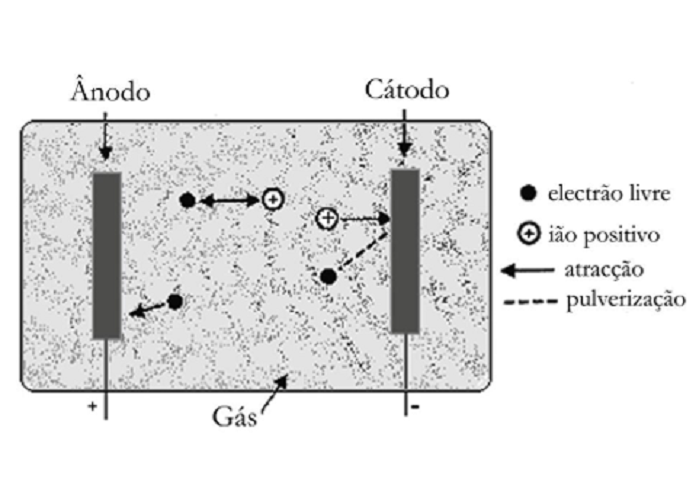
\includegraphics[width = 0.9\linewidth]{Figures/Cap2/GDOES_A_C.png}
      \caption{}
      \label{fig_GDOES_A_C}
    \end{subfigure}%
    \begin{subfigure}{.4\textwidth}
      \centering
      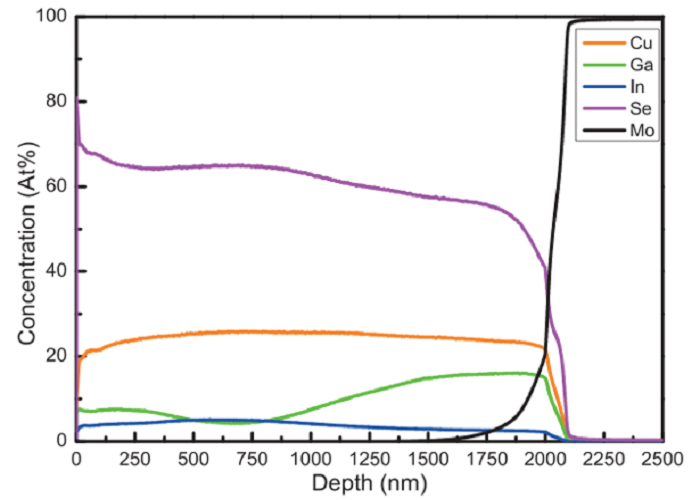
\includegraphics[width = 0.9\linewidth]{Figures/Cap2/GDOES_comp.png}
      \caption{}
      \label{fig:GDOES_comp}
    \end{subfigure}
    \caption[Funcionamento e resultados de um GDOES]%
    {À esquerda, Esquema de formação de um plasma GDOES, retirado de \cite{Santos2009}. À direita, Gráfico com resultado de uma espectroscopia, retirado de \cite{Covalent2022}.}
\end{figure}
%%%%%%%%%%%%%%%%%%%%%%%%%%%%%%%%%%%%%%%%%%%%%%%%%%%%%%%%%%%%%%%%%%%%%%%%%%%%%
\par
A luz emitida por este plasma secundário é coletada e o espectro formado é analisado. Cada elemento na amostra emite luz a um conjunto específico de comprimentos de onda, permitindo assim a determinação da composição elementar da amostra. A intensidade da emissão em cada comprimento de onda é proporcional à quantidade do elemento na amostra, permitindo uma análise quantitativa dos elementos presentes \cite{Saraiva2015}. Além disso, a composição elementar pode ser monitorizada ao longo do tempo, fornecendo um perfil de profundidade da composição do material, como pode ser visto na Figura \ref{fig:GDOES_comp}.
\par
Portanto, quando não se tem a certeza da composição química de uma liga metálica, por exemplo, após um tratamento de carbonitruração, pode-se realizar um ensaio de GDOES de forma a perceber a quantidade de carbono e azoto, e também outros elementos de liga, estão presentes no material, e as suas proporções em relação à profundidade.